% !TeX program = lualatex
\iffalse
Ignores everything in between. TODO list.

TODO

- 

\fi
%----------------------------------------------------------------------------------------
%
%	16-03-2024_technical_documentation.tex    										v.1.0
%	
%	Template for technical documentation for electronic devices.
%
%	M. Mojzis																   16.03.2024
%
%----------------------------------------------------------------------------------------
%	PREAMBULE
%----------------------------------------------------------------------------------------

\documentclass[a4paper, 10pt, twoside]{article}

\usepackage[left=2cm,includehead,headheight=1.3cm,top=1cm,right=2cm,bottom=2cm,bindingoffset=1cm,headsep=0.7cm]{geometry}

% Hyperlink referencing.
\usepackage[hyphens]{url}
\usepackage{hyperref}
% Page numbering in upper right corner.
\usepackage{fancyhdr}
% For title page.
\usepackage{setspace}
\usepackage{blindtext}
% TOC.
\usepackage{tocloft}
\usepackage{ragged2e}
% Images.
\usepackage{caption}
\usepackage{graphicx}
% Background image.
\usepackage{tikz}
\usepackage{eso-pic}	
\usepackage{multicol}
% Datetime package.
\usepackage{datetime}
\usepackage{etoolbox}

\usepackage{fontspec}
\usepackage{pdflscape}


%----------------------------------------------------------------------------------------
%	SETUP
%----------------------------------------------------------------------------------------
% Don't change if not needed.
%----------------------------------------------------------------------------------------
% Line spacing.
\linespread{1.25}
% Paragrph spacing.
\setlength{\parskip}{10pt}
% Break URLs.
\hypersetup{breaklinks=true}
% Image file path.
\graphicspath{ {./Figures/} }

% Add dots to TOC to all lines.
\renewcommand{\cftsecleader}{\cftdotfill{\cftdotsep}}
\renewcommand{\cftdotsep}{1}
\renewcommand{\cftbeforesecskip}{1pt}
% Remove name from TOC.
\renewcommand*\contentsname{}

% Page numbering.
\fancypagestyle{altstyle}
{
	% Clear the header and footer of any formating.
	\fancyhf{}
	
	% Include the logo and offset it from the top and add text, switch between odd pages.
	\fancyhead[RE,LO]{
\includegraphics[width=1cm]{logo}\\\textbf{www.github.com/matmoj04}}
	\fancyhead[RO,LE]{\textbf{SIMATIC S7-1200, KTP700 Basic}\\TDV01-MAREC 2024}
	
	% Make the line thicker.
	\renewcommand{\headrulewidth}{0.5mm}
	
	% Page numbering and altering the page orientation.
	\fancyfoot[RO,LE]{\small\thepage}
	\fancyfoot[LO,RE]{\small Copyright © 2024, Matej Mojžiš}
	
	\renewcommand{\footrulewidth}{0.5mm}
}

\fancypagestyle{fpstyle}
{
	% Clear the header and footer of any formating.
	\fancyhf{}
	
	% Include the logo and offset it from the top and add text, switch between odd pages.
	\fancyhead[RE,LO]{
\includegraphics[width=1cm]{logo}}
	\fancyhead[RO,LE]{\textbf{SIMATIC S7-1200, KTP700 Basic}\\TDV01-MAREC 2024}
	
	% Make the line thicker.
	\renewcommand{\headrulewidth}{0.5mm}
	
	% Page numbering and altering the page orientation.
	\fancyfoot[LE,RO]{}
	\fancyfoot[L]{
\includegraphics[width=1cm]{legal}Intellectual property of Matej Mojžiš, all rights reserved.}
	
	\renewcommand{\footrulewidth}{0.5mm}
}

\pagestyle{fpstyle}

\setmainfont{Arial}

%----------------------------------------------------------------------------------------

\begin{document}
%----------------------------------------------------------------------------------------
%	TITLE
%----------------------------------------------------------------------------------------

%----------------------------------------------------------------------------------------
{
	\center\LARGE\textbf{Didaktická pomôcka PLC}\\
	\noindent\rule{\textwidth}{0.5mm}
}
%----------------------------------------------------------------------------------------
%	VLASTNOSTI
%----------------------------------------------------------------------------------------

\begin{multicols}{2}
%----------------------------------------------------------------------------------------
{
	\section{Vlastnosti}
	
	\begin{itemize}
		\setlength\itemsep{0.1em}
		\item 
		\item 
		\item 
		\item 
		\item 
		\item 
	\end{itemize}
}
%----------------------------------------------------------------------------------------
%	APLIKÁCIE
%----------------------------------------------------------------------------------------
{
	\section{Aplikácie}
	
	\begin{itemize}
		\setlength\itemsep{0.1em}
		\item 
		\item 
		\item 
		\item 
		\item 
		\item 
	\end{itemize}
}
%----------------------------------------------------------------------------------------
%	POPIS
%----------------------------------------------------------------------------------------
{
	\section{Popis}
	
	Lorem ipsum dolor sit amet, consectetur adipiscing elit. Nam dui lectus, facilisis accumsan faucibus ac, lacinia ut lectus. Fusce molestie gravida fermentum. Duis tristique, orci vel aliquam porta, lacus lacus varius lectus, a consequat risus leo vel nulla. Fusce suscipit finibus sapien sed tincidunt. Nullam vitae lobortis felis, eget porttitor ligula. Nunc sagittis enim ut erat convallis, vel sagittis arcu pellentesque. Vestibulum condimentum lacus hendrerit orci eleifend, vitae dictum magna euismod. Maecenas leo nibh, scelerisque eget ornare vel, tristique in nibh. Cras malesuada non ante non pulvinar. In dui lorem, vehicula et dignissim ut, faucibus non mauris.
	
	Phasellus sollicitudin at ligula vitae convallis. Phasellus eros justo, convallis eu varius et, tincidunt et dolor. Interdum et malesuada fames ac ante ipsum primis in faucibus.
	
}
%----------------------------------------------------------------------------------------
\end{multicols}
%----------------------------------------------------------------------------------------
%	ZJEDNODUŠENÁ SCHĚMA
%----------------------------------------------------------------------------------------
{
	\section{Zjednodušená Schéma}
	
	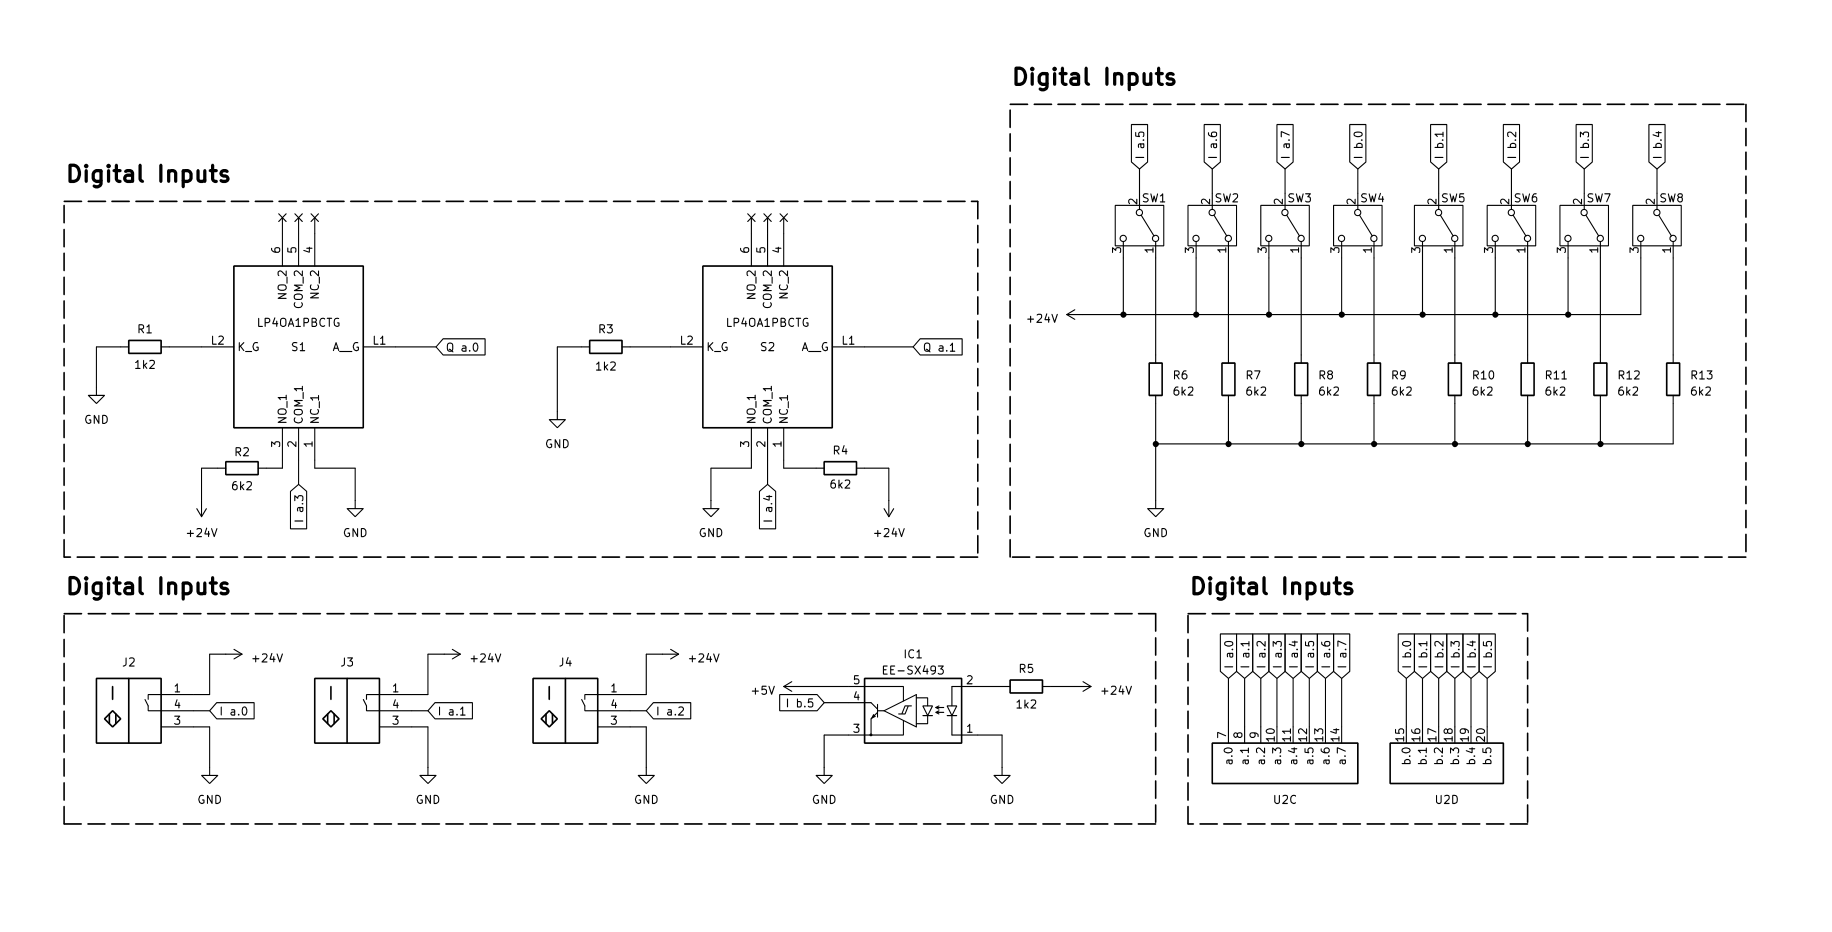
\includegraphics[width=\textwidth]{test}
}
%----------------------------------------------------------------------------------------
%	OBSAH
%----------------------------------------------------------------------------------------
\restoregeometry
\newpage
\pagestyle{altstyle}
\setcounter{page}{2}
\setlength{\columnsep}{1.5cm}
%----------------------------------------------------------------------------------------
{
	\newgeometry{left=2cm,includehead,headheight=1cm,top=1cm,right=2cm,bottom=3cm,bindingoffset=1.5cm,headsep=0.7cm}
	
	\fancyhfoffset[E,O]{0pt}
	
	\section*{\center{Obsah}}
	
	\begin{multicols}{2}
		\tableofcontents
		\thispagestyle{altstyle}
	\end{multicols}
	
	\noindent\rule{\textwidth}{0.5mm}
}
%----------------------------------------------------------------------------------------
%	REVÍZIA TECHNICKÉHO LISTU
%----------------------------------------------------------------------------------------
{
\section{Revízia Technického Listu}
}
%----------------------------------------------------------------------------------------
%	REVÍZIA VÝROBKU
%----------------------------------------------------------------------------------------
\restoregeometry
\newpage
%----------------------------------------------------------------------------------------
{
\subsection{Revízia Výrobku}
\begin{landscape}
	
\end{landscape}
}
%----------------------------------------------------------------------------------------
%	KONFIGURÁCIA A FUNKCIE PINOV 
%----------------------------------------------------------------------------------------
\newpage
%----------------------------------------------------------------------------------------
{
\section{Konfigurácia a funkcie vývodov}
}
%----------------------------------------------------------------------------------------
%	ŠPECIFIKÁCIE
%----------------------------------------------------------------------------------------
\newpage
%----------------------------------------------------------------------------------------
{
\section{Špecifikácie}
}

\end{document}
